\documentclass[letterpaper]{article}
\usepackage{amssymb}
\usepackage{fullpage}
\usepackage{changepage}
\usepackage{amsmath}
\usepackage{epsfig,float,alltt}
\usepackage{psfrag,xr}
\usepackage[T1]{fontenc}
\usepackage{url}
\usepackage{pdfpages}
\usepackage{epstopdf}
\usepackage[framed,numbered,autolinebreaks,useliterate]{mcode}

%\includepdfset{pagecommand=\thispagestyle{fancy}}
\author{Yi Yang}
\title{SEA Project Report 1}

\begin{document}
\date{09/19/2016}
\maketitle

\newcommand{\trace}{\mathrm{trace}}
\newcommand{\real}{\mathbb R}  % real numbers  {I\!\!R}
\newcommand{\nat}{\mathbb N}   % Natural numbers {I\!\!N}
\newcommand{\cp}{\mathbb C}    % complex numbers  {I\!\!\!\!C}
\newcommand{\ds}{\displaystyle}
\newcommand{\mf}[2]{\frac{\ds #1}{\ds #2}}
\newcommand{\spanof}[1]{\textrm{span} \{ #1 \}}
\newcommand{\sol}[0]{\textbf{Solution: }}
\newcommand{\pf}[0]{\textbf{Proof:}}
\newcommand{\rme}[0]{\textrm{e}}
\newcommand{\Null}[1]{\textrm{Null}\{#1\}}
\parindent 0pt
%%%%%%%%%%%%%%%%%%%%%%%%%%%%%%%%%%%%%%%%%%%%%%%%%%%%%%%%%%%%%%%%%%%%%%%%%%%%%%%
%report starts here!
%%%%%%%%%%%%%%%%%%%%%%%%%%%%%%%%%%%%%%%%%%%%%%%%%%%%%%%%%%%%%%%%%%%%%%%%%%%%%%%
This week, I re-plot driving point impedance theoretical results(virtual stiffness), codes and plots shown below:
\lstinputlisting[firstline=1, lastline=50]{thPlot.m}
\begin{figure}[H]
	\centering
	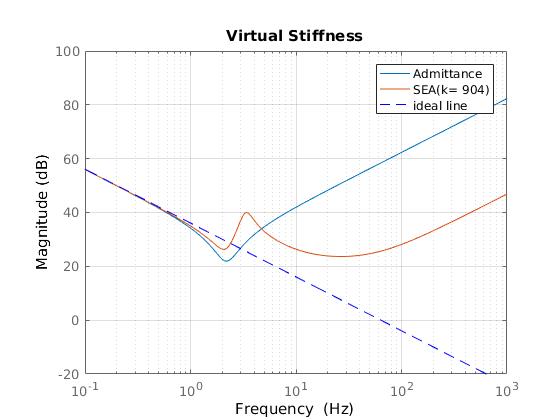
\includegraphics[scale=0.8]{theoretical.png}
	\caption{Driving point impedance theoretical results(virtual stiffness)}
	\label{fig:theo}
\end{figure}

After plotting the theoretical transfer function, I want to use some real data to estimate the transfer functions and compare them with the theoretical ones. First, I input a step signal with time step size $0.001s$, I add a white noise ($SNR = 10$) to the input signal and then apply it to the linear matlab model. By using \textit{tfestimate} function in Matlab, I can get the transfer function for admittance and SEA schemes respectively. The codes and plots are attached below:
\lstinputlisting[firstline=1, lastline=100]{sim_snr.m} 
\begin{figure}[H]
	\centering
	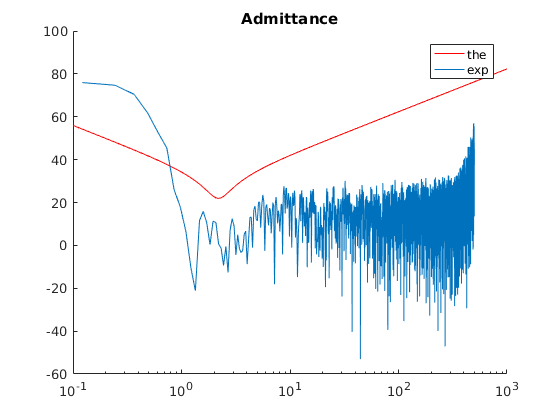
\includegraphics[scale=0.8]{admittance.png}
	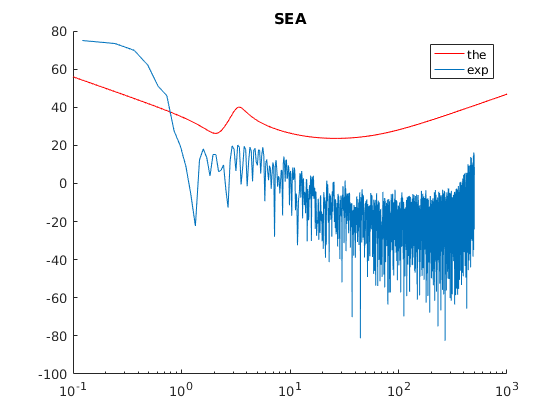
\includegraphics[scale=0.8]{sea.png}
\end{figure}
We can find that there is large discrepancy between theoretical curve and the curve generated by adding noise to the input signal. And I am not sure whether the method is correct to generate these results.\\


\vspace*{2cm}
\section*{Appendix}
System ID is shown below:
\lstinputlisting[firstline=1, lastline=50]{sysID.m}
\end{document}
